\documentclass[letterpaper, reqno,11pt]{article}
\usepackage[margin=1.0in]{geometry}
\usepackage{color,latexsym,amsmath,amssymb,graphicx, float}
\usepackage{hyperref}

\hypersetup{
colorlinks=true,
linkcolor=magenta,
filecolor=magenta,
urlcolor=cyan,
}

\graphicspath{ {images/} }

\newcommand{\RR}{\mathbb{R}}
\newcommand{\CC}{\mathbb{C}}
\newcommand{\ZZ}{\mathbb{Z}}
\newcommand{\QQ}{\mathbb{Q}}
\newcommand{\NN}{\mathbb{N}}
\newcommand{\st}{\text{ s.t.}\ }
\newcommand{\tn}[1]{\textnormal{#1}}
\newcommand{\m}{\textnormal{ m}}
\newcommand{\s}{\textnormal{ s}}
\newcommand{\K}{\textnormal{ K}}
\newcommand{\h}{\textnormal{ h}}
\newcommand{\W}{\textnormal{ W}}
\newcommand{\J}{\textnormal{ J}}
\newcommand{\Pa}{\textnormal{ Pa}}
\newcommand{\mol}{\textnormal{ mol}}
\newcommand{\Hz}{\textnormal{ Hz}}
\newcommand{\kg}{\textnormal{ kg}}
\newcommand{\cm}{\textnormal{ cm}}
\newcommand{\mm}{\textnormal{ mm}}
\newcommand{\N}{\textnormal{ N}}

\begin{document}
\pagenumbering{arabic}
\title{ELEC 221 Homework 2}
\date{October 13, 2021}
\author{Xander Naumenko}
\maketitle

{\noindent\bf Question 1a1.} $z_1+z_2=3+4e^{j\frac\pi4}=3+\frac4{\sqrt2}+j\frac4{\sqrt2}=(3+2\sqrt2)+j2\sqrt2=5.8284+2.8284j=6.48e^{0.451j}$

{\noindent\bf Question 1a2.} $\cos(\pi/4)-j\sin(\pi/4)+\frac{\sqrt2}2e^{j\frac\pi4}=0.707-0.707j+0.5+0.5=1.207-0.207j=1.225e^{-0.17j}$

{\noindent\bf Question 1b1.} $z_1z_2=12e^{j\frac\pi4}$

{\noindent\bf Question 1b2.} $z_1z_2=e^{-j\frac\pi4}\frac{\sqrt2}2e^{j\frac\pi4}=\frac{\sqrt2}{2}$

{\noindent\bf Question 1c1.} Let $z=a+bi$. Then 

$$
    \frac{(z+z*)}{2}=\frac{a+bj+a-bj}{2}=a=Re(z)
$$

{\noindent\bf Question 1c2.} Let $z=a+bi$. Then 

$$
    \frac{(z-z*)}{2j}=\frac{a+bj-a+bj}{2j}=b=\Im(z)
$$

{\noindent\bf Question 1c3.} Let $z=a+bi$. Then 

$$
    \sqrt{zz*}=\sqrt{(a+bi)(a-bi)}=\sqrt{a^2+b^2}=|z|
$$

{\noindent\bf Question 1d.} By definition, $z*=re^{-j\theta}$, so $\frac1{z*}=\frac1{re^{-j\theta}}=\frac1re^{j\theta}$ as desired. For the graphs see figure \ref{fig:1d}. 

\begin{figure}[htbp]
\centering
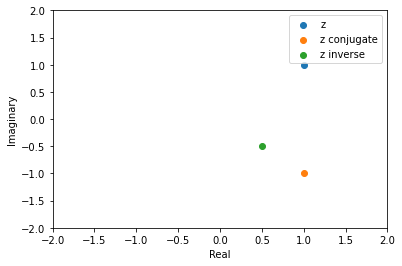
\includegraphics[width=\textwidth]{1d}
\caption{Graph for questio 1d}
\label{fig:1d}
\end{figure}

{\noindent\bf Question 1e.} Computing, we get 

$$
    {\bf B}^H=\begin{bmatrix}
        \cos(\pi/4)&0&e^{-j(\frac13+\frac\pi2)}\\
        e^j&2-3j&e^2
    \end{bmatrix}
$$

Similarly computing for $\bf v$, we get 

$$
    {\bf v}^H=
    \begin{bmatrix}
        1&
        e^{-j\pi/4}&
        e^{-j\pi/2}&
        e^{-j3\pi/4}
    \end{bmatrix}
$$

{\noindent\bf Question 2a.} Writing it out, we get 

$$
    {\bf \phi}=
    \begin{bmatrix}
        1&1&1&1\\
        1&e^{j(\pi/2)}&e^{j(\pi)}&e^{j3(\pi/2)}\\
        1&e^{j(\pi)}&e^{j2\pi}&e^{j3\pi}\\
        1&e^{j3(\pi/2)}&e^{j3\pi}&e^{j9(\pi/2)}
    \end{bmatrix}
$$

{\noindent\bf Question 2b.} By inspection, we find that 

$$
    x_m=e^{j(2\pi/N)(m-1)}
$$

{\noindent\bf Question 2c.} First note that because the matrix is symmetric about the diagonal, the transpose of the matrix is the matrix itself. Also since each entry has magnitude $1$, taking the conjugate of each entry just changes the sign in the exponent. Thus the entry in the $i$th row and $j$th column in the final resulting matrix will be the $i$th row dotted with the conjugates of the $j$th column. Writing this out in summation form we have 

$$
    [\Phi]^H[\Phi]_{m,l}=\sum_{n=1}^{N}e^{-j(2\pi/N)((m-1)(n-1)-(n-1)(l-1))}=\sum_{n=1}^{N}e^{j(2\pi(n-1)/N)(l-m)}
$$

If $l=m$, i.e. along the diagonals we have that the expression in the summation is just 1, so the diagonals have value $N$. If $l\neq m$, then let $r=e^{j(2\pi(n-1)/N)(l-m)}$ and using the geometric formula we find that 

$$
    [\Phi]^H[\Phi]_{m,l}=\frac{1-r^n}{1-r}=\frac{1-e^{j(2\pi(n-1)/N)(l-m)N}}{1-r}=\frac{1-e^{j(2\pi(n-1))(l-m)}}{1-r}=0
$$

This shows that all non-diagonal entries are 0, and the diagonals are non-zero so the matrix is diagonal. 

{\noindent\bf Question 2d.} Computing the dot product, we get 

$$
    \langle\phi_k, \phi_l\rangle=\sum_{n=1}^N e^{j(2\pi/N) k (n-1)}e^{-j(2\pi/N) l (n-1)}=\sum_{n=1}^N e^{j(2\pi/N) (k-l) (n-1)}
$$

If $k=l$, then the expression above becomes $N$. Otherwise, we again apply the geometric series and we see that 

$$
    \langle\phi_k, \phi_l\rangle=\frac{1-e^{j(2\pi) (k-l)}}{1-e^{j(2\pi/N) (k-l)}}=0
$$

Thus the inner product between each of the vectors is zero and they are all orthogonal to each other. 

{\noindent\bf Question 2e.} As we saw in the previous part, if $k=l$ (i.e. the vectors are the same) the result was of magnitude $N$, so to normalize them they would have to be divided by $\sqrt N$

{\noindent\bf Question 2f.} Since we know that ${\bf\Phi}^H{\bf\Phi}$ is a diagonal matrix, it must be the inverse of $\Phi$ up to a normalization. Since we found that the diagonals are $N$ we get that ${\bf\Phi}^{-1}=\frac1N{\bf\Phi^H}$. 

{\noindent\bf Question 2g.} Applying the inverse to both sides, we have 

$$
    \alpha={\bf\Phi}^H s
$$

{\noindent\bf Question 2h.} First note that $\alpha_k=\langle s, \phi_k\rangle$. Thus we can write $\alpha$ as a row vector as 

$$
    \alpha = \begin{bmatrix}\langle s, \phi_0\rangle&\ldots&\langle s, \phi_{N-1}\rangle\end{bmatrix}=\frac1N s\Phi^H
$$

Where $s$ is also represented as a row vector. Taking the inverse of both sides using the previous parts of this question, we get 

$$
    \alpha N\frac1N\Phi=\frac NNs\Phi^H\Phi=s
$$

Expanding the left side of this equation we get 

$$
    s=\alpha\Phi=\begin{bmatrix}\langle \alpha, \phi_0^*\rangle&\ldots&\langle \alpha, \phi_{n-1}^*\rangle\end{bmatrix}
$$

Looking at this row vector term by term, we find that 

$$
    s[n]=\langle\alpha, \phi_n^*\rangle=\sum_{k=0}^{N-1}\alpha_ke^{j(2\pi/N)kn}
$$

Since this is exactly what was desired in the question, we are done. 

{\noindent\bf Question 3a.} The support set is $\{0, 1, 2, 3, 4,\}$. The length of the signal is 5. 

{\noindent\bf Question 3b.} The support set of the impulse is $\{0, 1, 2, 3\}$. The order $M=4$.  

{\noindent\bf Question 3c.} The filter is causal because $h[n]=0\forall n<0$. 

{\noindent\bf Question 3d.} The length of the output is $M+N-1=8$. 

{\noindent\bf Question 3e.} The plot of their convulutions can be seen in figure \ref{fig:3e}. The computed values associated with the graph are as follows: 

$$
    y=[ 6, 10, 14, -4, 10,  4,  0,  2,  0]
$$

\begin{figure}[htbp]
\centering
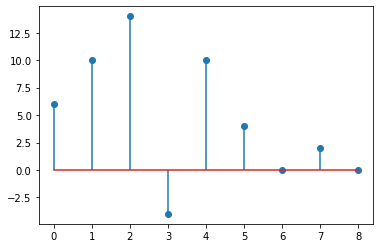
\includegraphics[width=\textwidth]{3e}
\caption{Plot for question 3e. }
\label{fig:3e}
\end{figure}

{\noindent\bf Question 5a.} See figure \ref{fig:5a}. 

\begin{figure}[htbp]
\centering
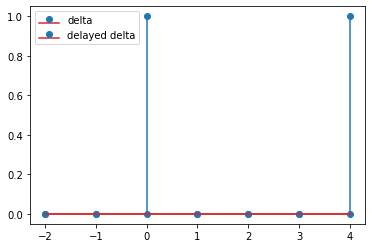
\includegraphics[width=\textwidth]{5a}
\caption{Figure for question 5a}
\label{fig:5a}
\end{figure}

{\noindent\bf Question 5b.} Let $n, l\in\ZZ$. If $n\neq l$, then $s[n]\delta[n-\ell]=s[n](0)=0=s[\ell]\delta[n-\ell]$. If $n=l$, then we have $s[n]\delta[n-\ell]=s[n]\delta[0]=s[n]=s[\ell]=s[\ell]\delta[0]$. In either case theyr'e the same so we're done. 

{\noindent\bf Question 5c.} Doing the sum, we get 

$$
    \sum_{\ell\in\ZZ}s[n]\delta[n-\ell]=s[n]\delta[0]+\sum_{\ell\in\ZZ,\ell\neq0}s[\ell]\cdot 0=s[n]
$$

{\noindent\bf Question 5d.} Applying part b to the summand, we get 

$$
    \sum_{\ell\in\ZZ} s[\ell]\delta[n-\ell]=\sum_{\ell\in\ZZ}s[n]\delta[n-\ell]
$$

By part c this simplifies to $s[n]$ so we're done. 

{\noindent\bf Question 5e.} Let the system be $T$. Using part d, we have that 

$$
    s[n]=\sum_{\ell\in\ZZ}s[\ell]\delta[n-\ell]
$$

$$
    T(s[n])=y[n]=\sum_{\ell\in\ZZ}s[\ell]T(\delta[n-\ell])=\sum_{\ell\in\ZZ}s[\ell]h_\ell[n]
$$

The last step was because by definition, $T(\delta[n-\ell])=h_\ell[n]$. 

{\noindent\bf Question 5f.} Because the system is time invariant, it's impulse response to $\delta[n-\ell]=\delta[n]\forall\ell\in\ZZ$. This means that all of the $h_k$s are the same, i.e. $\exists h\st h_k[n]=h[n]\forall k$. Then applying part e, we have that 

$$
    y[n]=\sum_{k\in\ZZ}s[k]h_k[n-k]\sum_{k\in\ZZ}s[k]h[n-k]
$$

as required. 

{\noindent\bf Question 5g.} See figures \ref{fig:5gi} and \ref{fig:5gii}. 

\begin{figure}[htbp]
\centering
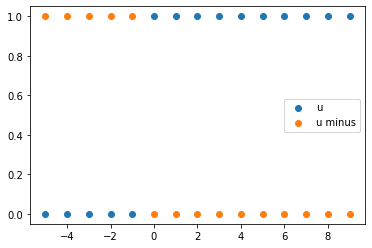
\includegraphics[width=\textwidth]{5gi}
\caption{Graph for question 5g}
\label{fig:5gi}
\end{figure}

\begin{figure}[htbp]
\centering
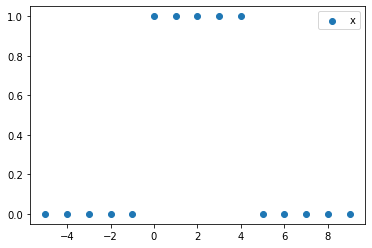
\includegraphics[width=\textwidth]{5gii}
\caption{Graph for question 5g}
\label{fig:5gii}
\end{figure}

\end{document}